\documentclass[10pt]{article}

%Math
\usepackage{amsmath}
\usepackage{amsfonts}
\usepackage{amssymb}
\usepackage{amsthm}
\usepackage{ulem}
\usepackage{stmaryrd} %f\UTF{00FC}r Blitz!

%PageStyle
\usepackage[ngerman]{babel} % deutsche Silbentrennung
\usepackage[utf8]{inputenc} 
\usepackage{fancyhdr, graphicx}
\usepackage[scaled=0.92]{helvet}
\usepackage{enumitem}
\usepackage{parskip}
\usepackage[a4paper,top=2cm]{geometry}
\setlength{\textwidth}{17cm}
\setlength{\oddsidemargin}{-0.5cm}


% Shortcommands
\newcommand{\Bold}[1]{\textbf{#1}} %Boldface
\newcommand{\Kursiv}[1]{\textit{#1}} %Italic
\newcommand{\T}[1]{\text{#1}} %Textmode
\newcommand{\Nicht}[1]{\T{\sout{$ #1 $}}} %Streicht Shit durch

%Arrows
\newcommand{\lra}{\leftrightarrow} 
\newcommand{\ra}{\rightarrow}
\newcommand{\la}{\leftarrow}
\newcommand{\lral}{\longleftrightarrow}
\newcommand{\ral}{\longrightarrow}
\newcommand{\lal}{\longleftarrow}
\newcommand{\Lra}{\Leftrightarrow}
\newcommand{\Ra}{\Rightarrow}
\newcommand{\La}{\Leftarrow}
\newcommand{\Lral}{\Longleftrightarrow}
\newcommand{\Ral}{\Longrightarrow}
\newcommand{\Lal}{\Longleftarrow}

% Code listenings
\usepackage{color}
\usepackage{xcolor}
\usepackage{listings}
\usepackage{caption}
\DeclareCaptionFont{white}{\color{white}}
\DeclareCaptionFormat{listing}{\colorbox{gray}{\parbox{\textwidth}{#1#2#3}}}
\captionsetup[lstlisting]{format=listing,labelfont=white,textfont=white}
\lstdefinestyle{JavaStyle}{
 language=Java,
 basicstyle=\footnotesize\ttfamily, % Standardschrift
 numbers=left,               % Ort der Zeilennummern
 numberstyle=\tiny,          % Stil der Zeilennummern
 stepnumber=5,              % Abstand zwischen den Zeilennummern
 numbersep=5pt,              % Abstand der Nummern zum Text
 tabsize=2,                  % Groesse von Tabs
 extendedchars=true,         %
 breaklines=true,            % Zeilen werden Umgebrochen
 frame=b,         
 %commentstyle=\itshape\color{LightLime}, Was isch das? O_o
 %keywordstyle=\bfseries\color{DarkPurple}, und das O_o
 basicstyle=\footnotesize\ttfamily,
 stringstyle=\color[RGB]{42,0,255}\ttfamily, % Farbe der String
 keywordstyle=\color[RGB]{127,0,85}\ttfamily, % Farbe der Keywords
 commentstyle=\color[RGB]{63,127,95}\ttfamily, % Farbe des Kommentars
 showspaces=false,           % Leerzeichen anzeigen ?
 showtabs=false,             % Tabs anzeigen ?
 xleftmargin=17pt,
 framexleftmargin=17pt,
 framexrightmargin=5pt,
 framexbottommargin=4pt,
 showstringspaces=false      % Leerzeichen in Strings anzeigen ?        
}

%Config
\renewcommand{\headrulewidth}{0pt}
\setlength{\headheight}{15.2pt}

%Metadata
\title{
	\vspace{5cm}
	Uebung 5 Dokumentation
}
\author{Jonas Schwammberger}
\date{5. Semester (HS 2013)}


% hier beginnt das Dokument
\begin{document}

% Titelbild
\maketitle
\thispagestyle{fancy}

\newpage

% Inhaltsverzeichnis
\pagenumbering{Roman}
\tableofcontents	  	


\newpage
\setcounter{page}{1}
\pagenumbering{arabic}

% Inhalt Start

\section{Einleitung}

\section{Algorithmus für die konvexe Hülle}
Für die Berechnung der konvexen Hülle standen zwei Algorithmen zur Verfügung. Der Algorithmus von Graham und von Jarvis March. Welcher Algorithmus (O(n log n) versus O(n*m)) besser ist, hängt vom Eingabeverhalten des Benutzers ab. Da ich zum durchschnittlichen Verhalten keine Daten habe wurde Graham ausgewählt. Der Algorithmus von Graham wurde aus interesse von mir selber implementiert und modifiziert.

\subsection{Modifikation}
Die Modifikation beschränkt sich darauf, dass nach dem Abbrechen der Hauptschleife nochmals eine isConvex() Prüfung mit Punkt $P_{0}$, $P_N$ und $P_{N-1}$. Im falle das $P_N$ auf der Strecke zwischen $P_{0}$ und $P_{N-1}$ ist  $P_N$ nicht in der minimalen konvexen Hülle. Dies prüft der Algorithmus von Graham nicht, deshalb wurde diese Modifikation vorgenommen.

\section{Algorithmus für die Berechnung des minimalen Rechtecks}
Gegeben sei die konvexe Hülle einer Punktmenge, von der das minimale Rechteck berechnet werden soll.
\begin{enumerate}
	\item Erstelle ein achsenparalelles Rechteck um die konvexe Hülle. Jede Seite berührt die konvexe Hülle in einem Punkt.
	\item Drehe alle Seiten des Rechtecks um den Berührungspunkt.
	\item Wenn sich eine Seite mit einem weiteren Punkt berührt, ist das eine mögliche Lösung.
	\item Fahre mit Schritt 2 weiter, jedoch soll sich die Seite nun um den neuen Berührungspunkt drehen.
\end{enumerate}
Das wird durchgeführt, bis der totale Winkel, mit dem das Rechteck gedreht wurde, mindestens 90$^\circ$ ist.

Der Algorithmus braucht mindestens vier Punkte, deshalb muss beim Input von drei Punkten eine Sonderbehandlung durchgeführt werden.

\subsection{Sonderbehandlung bei drei Punkten}
Bei drei Punkten muss man nur das minimale Rechteck eines Dreiecks finden. Das minimale Rechteck liegt immer mit einer seite an der längsten Seite des Dreiecks.

\subsection{Implementation}
\subsubsection{ModifiedGraham}
\subsubsection{SmallestRectangle}
\subsubsection{Line}
\subsubsection{Vector}

\subsection{Fazit}
Die totale Laufzeit des Algorithmus setzt sich aus zwei Laufzeiten zusammen
\begin{enumerate}
 \item Laufzeit für das finden der konvexe Hülle.
 \item Laufzeit für das finden des minimalen Rechtecks.
\end{enumerate}
Die Laufzeit vom Graham-Algorithmus ist bekannt, $O(n log(n))$. Die Laufzeit für das minimale Rechteck setzt sich wie folgt zusammen:
\begin{itemize}
 \item Nächsten Berührungspunkt finden. Der nächst mögliche Berührungspunkt einer Geraden ist der Index (in der konvexen Hülle) des momentanen Berührungspunktes +1 (-1 wenn man im Gegenuhrzeigersinn dreht). Das ergibt eine Laufzeit von $O(1)$, falls man die 4 Indizes speichert.
 \item Die vier Winkel für die nächsten Berührungspunkte berechnen, den Kleinsten auswählen und die Geraden drehen. Es bleiben immer vier Geraden deshalb $O(1)$
 \item Flächenberechnung braucht ebenfalls keine Schleife, deshalb $O(1)$
\end{itemize}
Das wird solange ausgeführt, bis der totale Winkel 90$^\circ$ ist. Das ist genau dann der Fall, wenn jeder Punkt in der konvexen Hülle genau ein Mal ein Berührungspunkt einer Geraden war. Das ergibt eine Laufzeit von $O(m)$ (m sei die Anzahl der Punkte der konvexen Hülle).

Der grösste Nachteil dieser Implementierung ist, dass für die Drehung Floating Point Datentypen verwendet werden müssen. Bei der Konvertierung von Floating Point zu Integer kommen oft Fehler von +-1 vor, welches auf der Graphik sofort Sichtbar ist. 

\begin{figure} [h!]

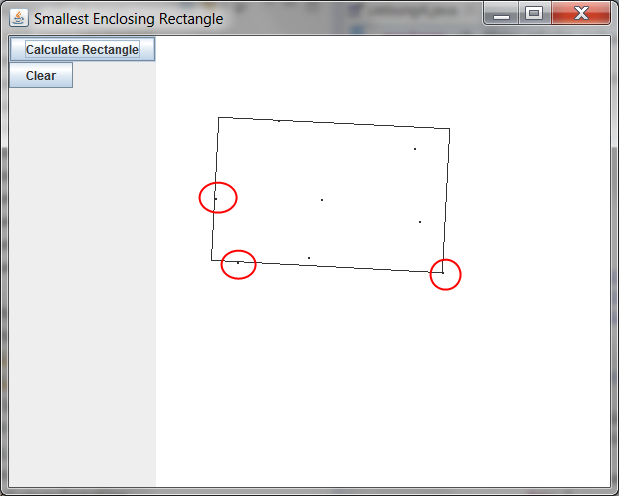
\includegraphics[scale= 0.75]{screenshot.png}
\caption{Fehler durch Floating Point Rundung}
\end{figure}

Ein vielleicht genauerer Ansatz wäre, eine Gerade an eine Seite der konvexen Hülle zu legen und daraus das minimale Dreieck berechnen. Wenn man das für die Hälfte aller Seiten durchführt, erhält man ebenfalls das minimale Rechteck. Jedoch muss man alleine für die Paralelle den Punkt mit dem grössten Abstand zur geraden finden, welches einen Aufwand von $O(m)$ pro Seite bedeutet (m sei die Anzahl der Punkte der konvexen Hülle). Wenn man den Algorithmus für ca $m/2$ Punkte ausführt, ergibt das eine Laufzeit von $O(m^2)$, was ebenfalls nicht erwünschenswert ist.
% Inhalt Ende 
\end{document} 